
\documentclass[10pt,twocolumn,letterpaper,bold]{article}

\usepackage[pagenumbers]{cvpr} %

\newcommand{\red}[1]{{\color{red}#1}}
\newcommand{\todo}[1]{{\color{red}#1}}
\newcommand{\TODO}[1]{\textbf{\color{red}[TODO: #1]}}

\definecolor{junglegreen}{rgb}{0.113, 0.639, 0.5}
\newcommand{\mhc}[1]{{\color{junglegreen}{\textbf{Marc: #1}}}}
\newcommand{\mhr}[2]{{\color{junglegreen}{\st{#1} #2}}}
\newcommand{\mhe}[1]


\newcommand{\methodterm}{BME1102\xspace}

\definecolor{cvprblue}{rgb}{0.21,0.49,0.74}

\definecolor{custompink}{RGB}{255, 0, 144}  %

\newcommand{\myparagraph}[1]{\vspace{0.1em}\noindent\textbf{#1}}

\usepackage[pagebackref,breaklinks,colorlinks,allcolors=cvprblue]{hyperref}
\newcommand{\jyh}[1]{{\color{blue} #1}}
\usepackage{multirow}
\def\paperID{5019} %
\def\confName{CVPR}
\def\confYear{2025}



 \title{Multi-contrast MRI Reconstruction from Undersampled Data}


\author{
    Yiwen Cai$^*$ \\
    Shanghaitech University \\
    2023533145 \\
    {\tt\small caiyw2023@shanghaitech.edu.cn}
    \and
    Zidong Song$^*$ \\
    Shanghaitech University \\
    2024533002 \\
    {\tt\small songzd2024@shanghaitech.edu.cn}
    \and % 如果这里没有自动换行形成 2x2，可以在 \and 前面加上 \\[10pt]
    Jingxuan Zhang$^*$ \\
    Shanghaitech University \\
    2023533003 \\
    {\tt\small zhangjx12023@shanghaitech.edu.cn}
    \and
    Yatu Zhang$^*$ \\
    Shanghaitech University \\
    2023533005 \\
    {\tt\small zhangyt2023@shanghaitech.edu.cn}
}

\usepackage{colortbl}
\newcommand{\highlightBest}[1]{\colorbox[rgb]{.866,.945, 0.831}{#1}}
\newcommand{\bestCellColor}[1]{\cellcolor[rgb]{.866,.945, 0.831}#1}

\newcommand{\highlightSecondBest}[1]{\colorbox[rgb]{1, 0.98, 0.83}{#1}}
\newcommand{\secondBestCellColor}[1]{\cellcolor[rgb]{1, 0.98, 0.83}#1}
\newcommand{\highlightThirdBest}[1]{\colorbox[rgb]{1, 0.87, 0.85}{#1}}
\newcommand{\thirdBestCellColor}[1]{\cellcolor[rgb]{1, 0.87, 0.85}{#1}}
\begin{document}

\maketitle
\def\thefootnote{*}\footnotetext{Equal Contribution. }



\section{Introduction}
In clinical Magnetic Resonance Imaging (MRI), reducing scan time is crucial for patient comfort and minimizing motion artifacts \cite{lustig2007sparse}. However, accelerating MRI scans by undersampling in k-space inevitably leads to severe aliasing artifacts in the reconstructed images. To recover high-quality, aliasing-free images while maintaining high acceleration factors, deep learning approaches have shown tremendous potential and superiority over traditional compressed sensing methods \cite{schlemper2017deep, wang2016accelerating}. This project aims to utilize the BraTS (Brain Tumor Segmentation) dataset to develop a robust, deep learning-based MRI reconstruction algorithm.

In the initial phase (Task 2), we implemented a baseline reconstruction network employing a standard U-Net architecture \cite{ronneberger2015u}. This model was trained using an L2 loss (Mean Squared Error) objective to minimize the pixel-wise discrepancy between the reconstructed image and the fully sampled ground truth. However, an in-depth analysis of the baseline results revealed that relying solely on L2 loss constraints inherently causes the network to generate over-smoothed images, resulting in the loss of critical high-frequency edges and fine texture details during reconstruction \cite{johnson2016perceptual}.

More importantly, we observed a significant limitation during evaluation: reconstructed images with a higher Peak Signal-to-Noise Ratio (PSNR) do not necessarily exhibit better image quality from a human visual perspective. To thoroughly investigate and validate this phenomenon, drawing inspiration from studies on image sharpness, we designed and conducted a ``shifting pixels'' experiment. The experimental results compellingly demonstrated that when an image undergoes a minor spatial shift, the PSNR drops drastically, yet the subjective image quality perceived by the human eye remains completely unchanged. This underscores the severe flaws of traditional pixel-wise metrics in reflecting true visual fidelity \cite{ledig2017photo}.

Based on these observations, we made the following core contributions in the advanced reconstruction phase of this project:
\begin{itemize}
    \item \textbf{Integration of Wavelet Loss:} To address the over-smoothing issue in the U-Net baseline, we introduced a wavelet loss constraint in the frequency domain. This structural penalty enables the network to better focus on and recover the high-frequency details of the image \cite{kang2018deep}.
    \item \textbf{Introduction of DISTS Metric and Perceptual Loss:} To tackle the misalignment between PSNR and human visual perception, we incorporated the Deep Image Structure and Texture Similarity (DISTS) metric into our evaluation framework, which explicitly focuses on texture and structural fidelity \cite{ding2020image}. Concurrently, we integrated a perceptual loss into our training objectives \cite{johnson2016perceptual}. This guides the network to approximate the ground truth at the feature level rather than merely the pixel level, significantly enhancing subjective visual quality.
    \item \textbf{Multi-modal Fusion and Unrolled Reconstruction:} To achieve clinical-grade quality, we developed a sophisticated multi-modal fusion architecture in Task 3. This design takes two modalities as input: an undersampled T2 image and a fully sampled T1 image, leveraging the anatomical structural prior from T1 to help recover T2 details \cite{zhou2020dudornet}. Furthermore, we implemented an unrolled reconstruction network by cascading the denoising network with Data Consistency (DC) layers to strictly ensure k-space fidelity \cite{schlemper2017deep}.
\end{itemize}

Ultimately, we seamlessly integrated the wavelet loss and perceptual loss into the training of the multi-modal unrolled network. Experimental results prove that our complete pipeline not only achieves excellent performance in quantitative metrics but also makes significant breakthroughs in preserving tumor details and eliminating aliasing artifacts visually.







\section{Method}\label{sec:algorithm} 

\subsection{Data Processing and Undersampling Simulation}
To train our reconstruction networks, we first need to simulate the k-space undersampling process that occurs in accelerated clinical MRI scans. As illustrated in Figure \ref{fig:undersampling}, we start with fully sampled 2D image slices. We apply a 2D Fast Fourier Transform (FFT) to convert these images into the frequency domain (k-space). Subsequently, we generate a 2D random variable-density undersampling mask with a specific acceleration factor (e.g., $5\times$). This mask is applied to the fully sampled k-space data to simulate the acquisition process. Finally, an Inverse Fast Fourier Transform (IFFT) is applied to the undersampled k-space data to obtain the zero-filled, aliased images, which serve as the inputs to our deep learning models.

\begin{figure}[h]
    \centering
    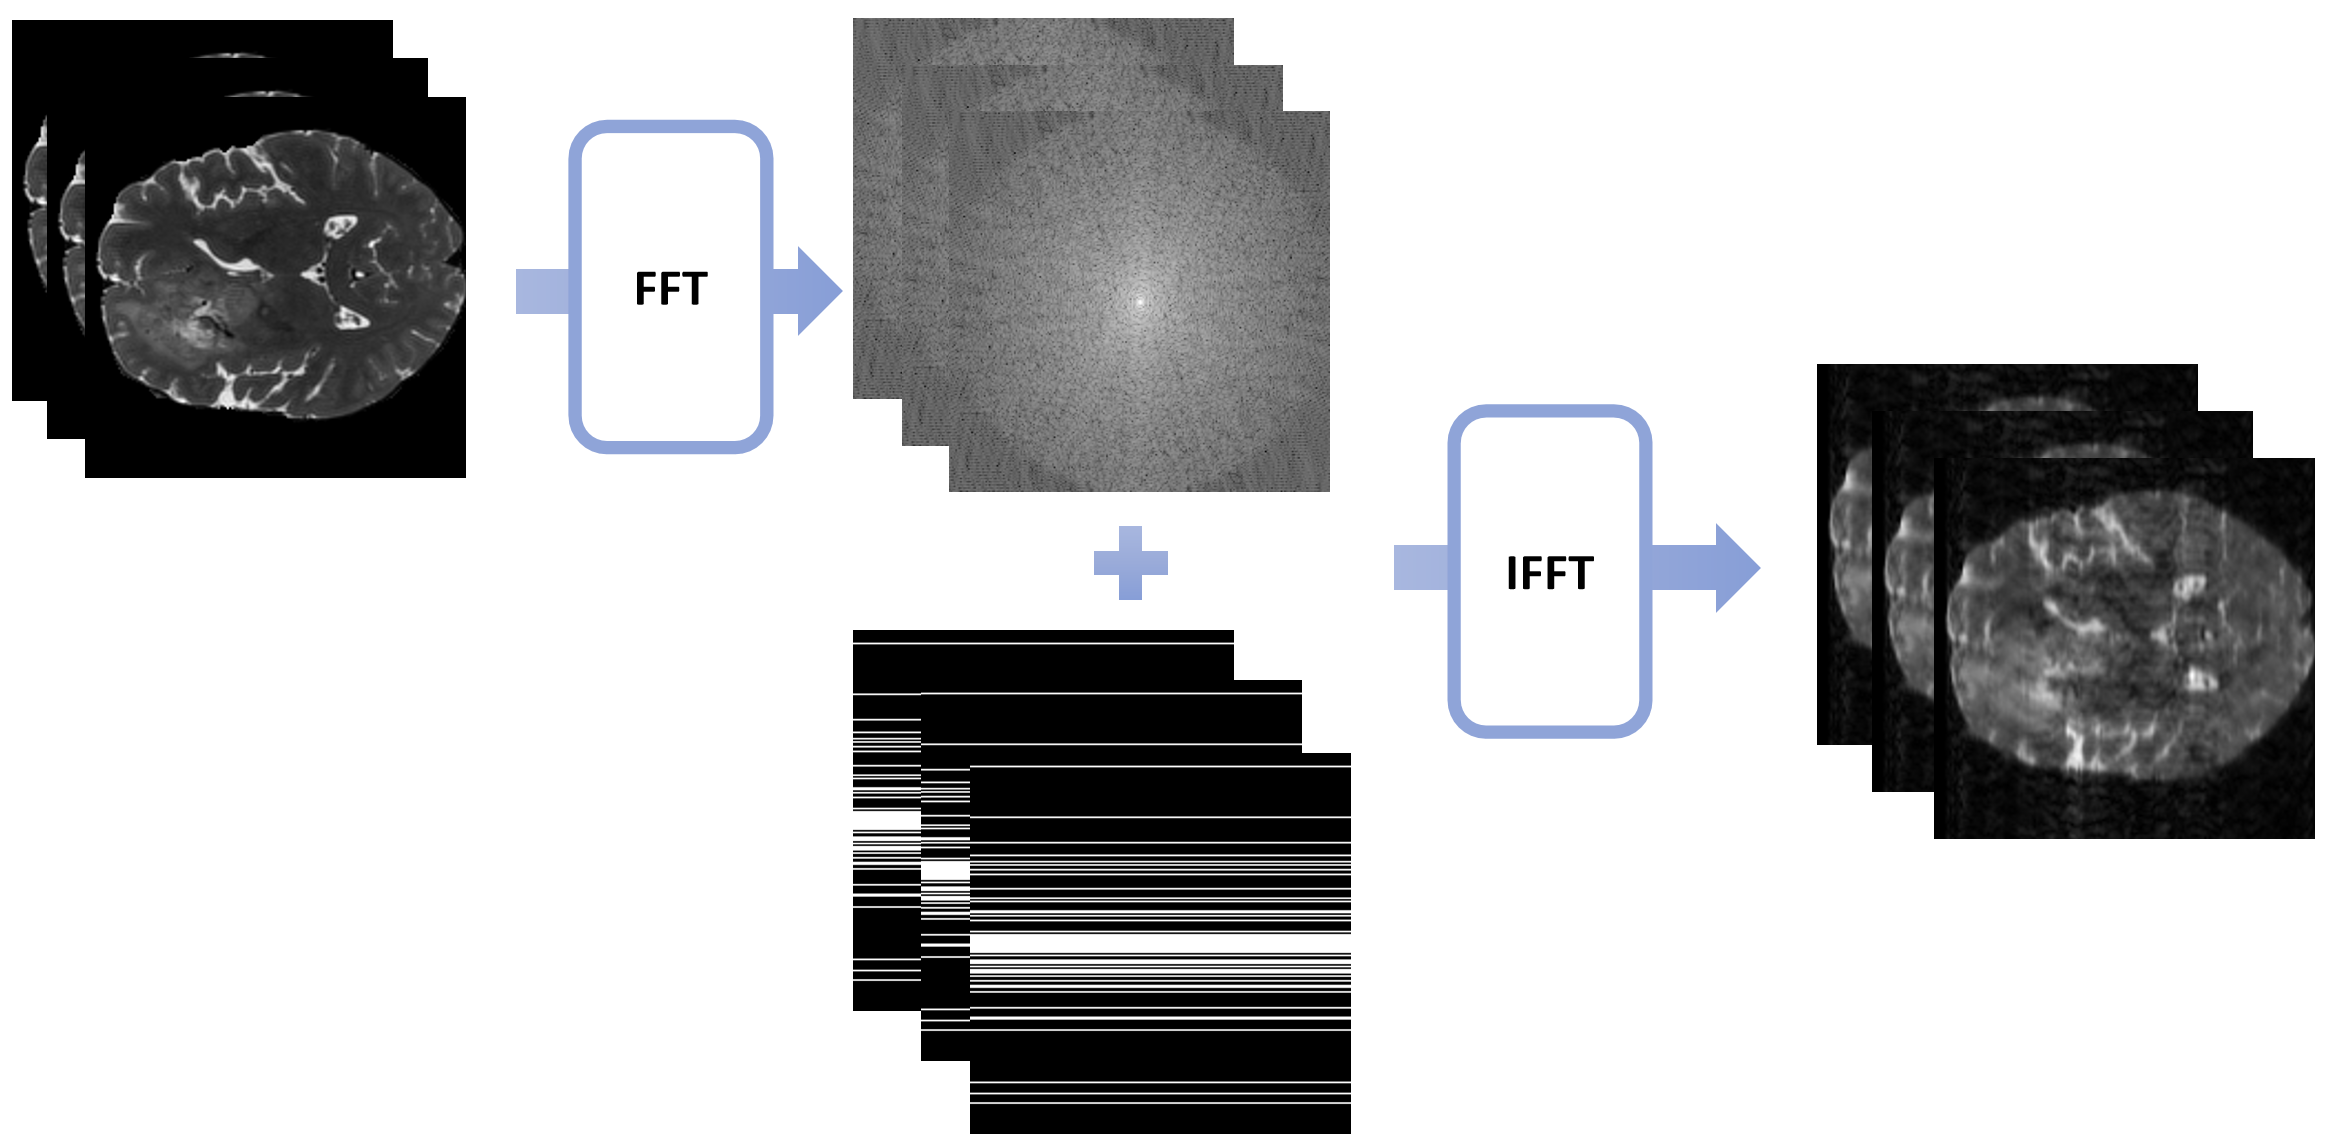
\includegraphics[width=\linewidth]{figures/data.png}
    \caption{Pipeline of the data preprocessing and undersampling simulation}
    \label{fig:undersampling}
\end{figure}

\subsection{Baseline Reconstruction Network (Task 2)}
In the initial phase of our project, we formulated the MRI reconstruction as an image-to-image translation problem and developed a baseline model based on the U-Net architecture, as shown in Figure \ref{fig:task2_unet}. The network takes the blurred, undersampled MRI image as input and processes it through a symmetric encoder-decoder structure. 

The encoder progressively downsamples the spatial resolution while increasing the channel depth using DoubleConv blocks (a sequence of $3\times3$ Convolution, Batch Normalization, and ReLU activation) followed by Max Pooling layers. A bottleneck layer captures the deepest latent representations. The decoder then progressively upsamples the feature maps using Transposed Convolutions and fuses them with high-resolution features from the encoder via skip connections. A final $1\times1$ convolution maps the deep features back to a single-channel reconstructed MRI image.
\begin{figure*}[t] 
	\begin{center} 
		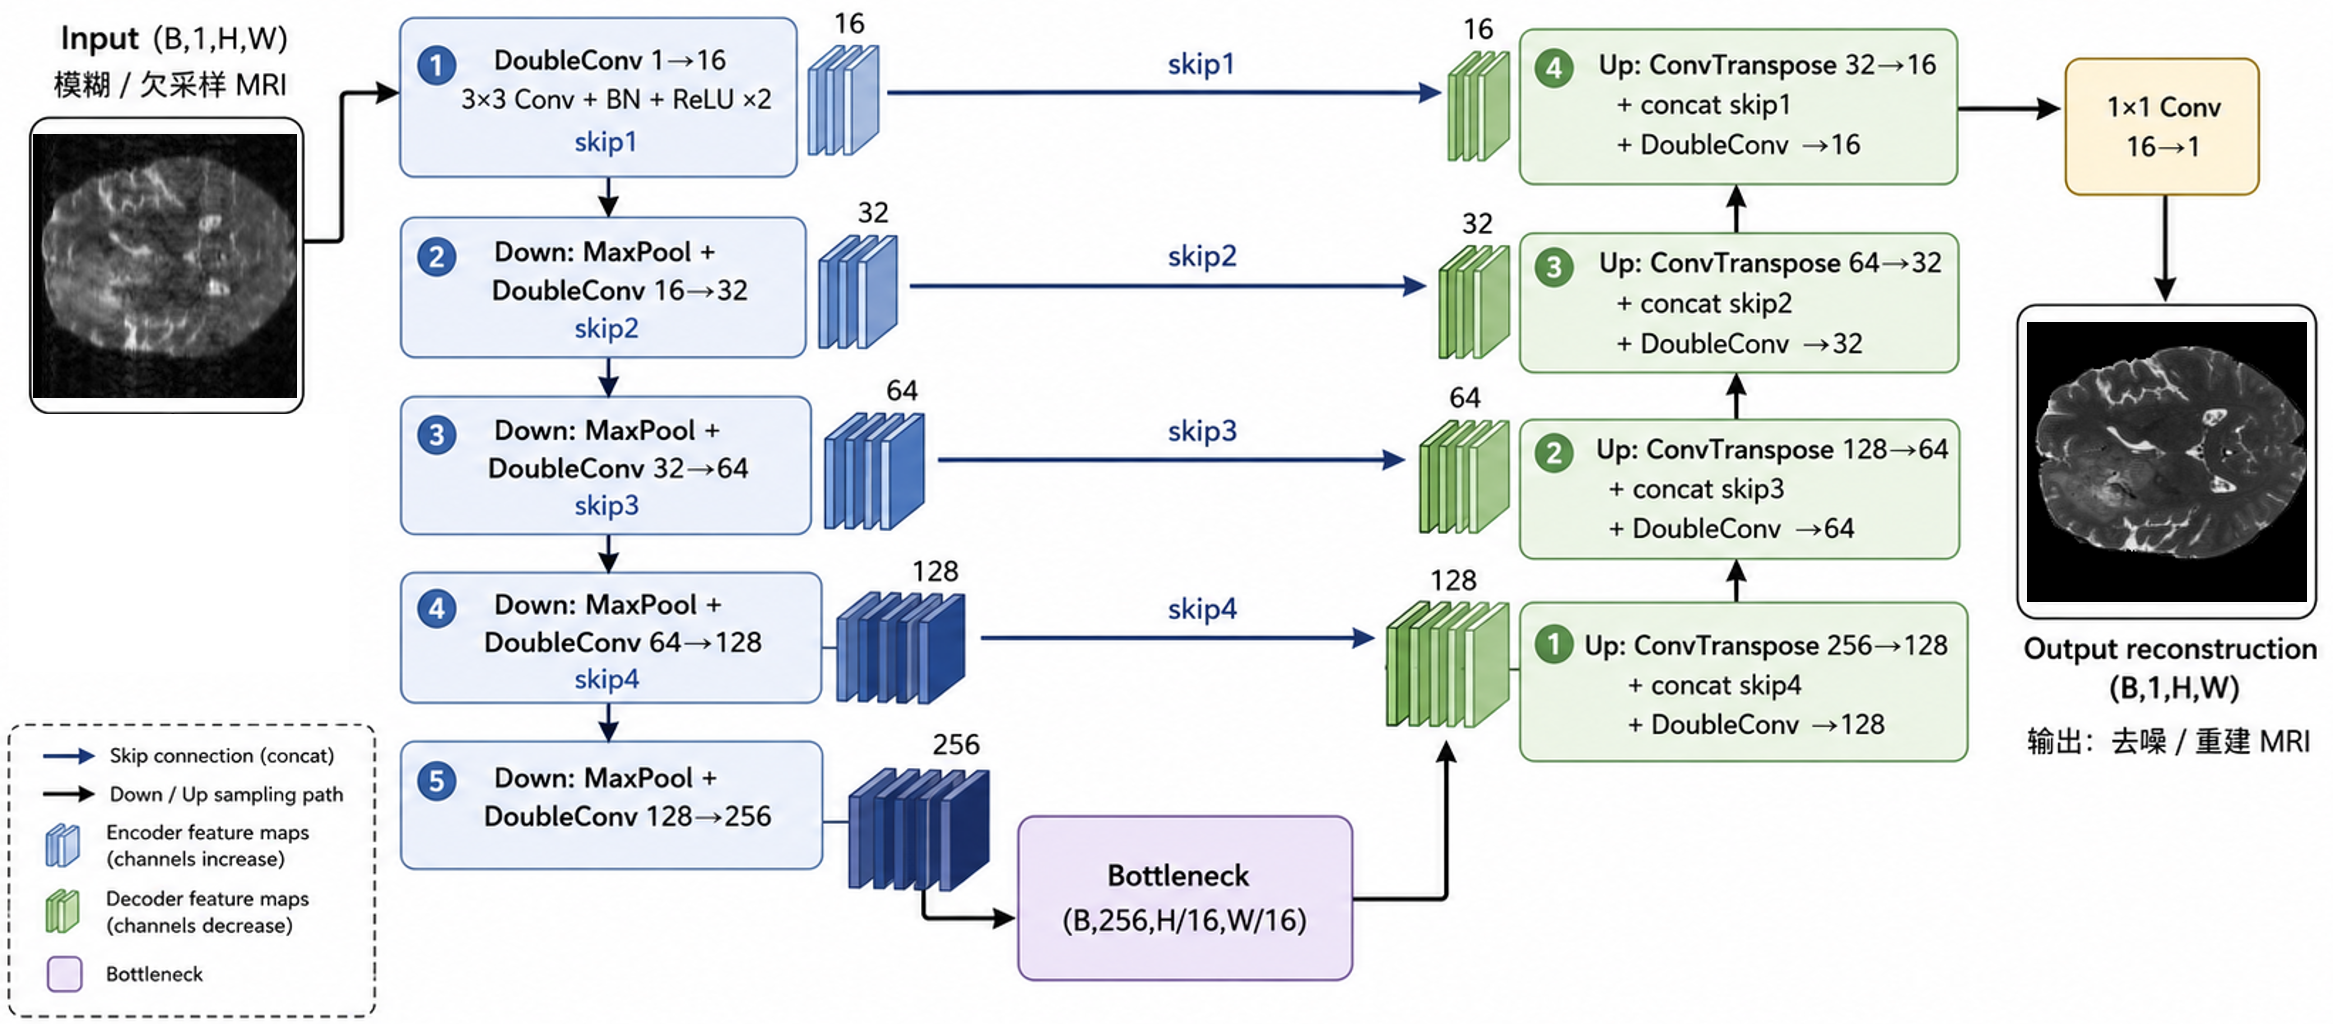
\includegraphics[width=\linewidth]{figures/pipeline_1.png} 
	\end{center} 
    \vspace{-20pt}  
	\caption{Overall pipeline of the baseline U-Net architecture (Task 2), which employs a symmetric encoder-decoder structure with skip connections to reconstruct high-quality, aliasing-free MRI images from undersampled T2 inputs.}
	\label{fig:task2_unet} 
	\vspace{-15pt}
\end{figure*} 


\subsection{Multi-modal Fusion and Unrolled Reconstruction (Task 3)}
To further elevate the reconstruction quality to a clinical grade, we advanced our architecture to a Multi-modal Unrolled Reconstruction Network (Figure \ref{fig:task3_pipeline}). This advanced pipeline leverages the fully sampled T1 modality to guide the reconstruction of the highly undersampled T2 modality.

The architecture consists of three core components:
\begin{enumerate}
    \item \textbf{Feature Fusion Module:} We utilize shallow CNN encoders to extract features from both the aliased T2 image and the fully sampled T1 image. A Cross-Attention mechanism is introduced where the T2 features act as the \textit{Query}, and the T1 features act as the \textit{Key} and \textit{Value}. This allows the network to borrow structural priors from the T1 image to complement the missing information in T2.
    \item \textbf{Unrolled Block:} The fused features are fed into a cascade of iterative unrolled blocks. Each block mimics an iteration of traditional optimization algorithms, containing a CNN Denoiser/Regularizer to refine the image features recursively.
    \item \textbf{Data Consistency (DC) Layer:} To ensure fidelity to the originally acquired data, a DC layer is appended after each unrolled iteration. It transforms the intermediate prediction back to the k-space, replaces the predicted values at sampled positions with the actual measured k-space data, and transforms it back to the image domain.
\end{enumerate} 

\subsection{Loss Function Design}
Traditionally, MRI reconstruction models are optimized using solely the Mean Squared Error (MSE) loss. However, relying purely on pixel-wise loss functions often leads to over-smoothed results. To mitigate this and enhance both the structural fidelity and visual quality, we formulated a comprehensive hybrid loss function combining MSE, Wavelet, and Perceptual losses:
\begin{equation}
\begin{split}
    \mathcal{L}_{total} &= \lambda_{mse}\mathcal{L}_{MSE}(x, \hat{x}) \\
    &\quad + \lambda_{wavelet}\mathcal{L}_{Wavelet}(x, \hat{x}) \\
    &\quad + \lambda_{perceptual}\mathcal{L}_{LPIPS}(x, \hat{x})
\end{split}
\end{equation}
where $x$ is the ground truth fully sampled image, $\hat{x}$ is the reconstructed image, and $\lambda$ represents the balancing weights for each respective component.

\textbf{Wavelet Loss ($\mathcal{L}_{Wavelet}$):} We introduced a wavelet-domain loss to explicitly penalize the loss of high-frequency details. By decomposing the images into four frequency bands using the Discrete Wavelet Transform, we calculate the $L_1$ distance for each band separately:
\begin{equation}
\begin{split}
    \mathcal{L}_{wavelet} &= w_{LL}\|LL_x - LL_{\hat{x}}\|_1 + w_{LH}\|LH_x - LH_{\hat{x}}\|_1 \\
    &\quad + w_{HL}\|HL_x - HL_{\hat{x}}\|_1 + w_{HH}\|HH_x - HH_{\hat{x}}\|_1
\end{split}
\end{equation}
Here, the $LL$ band preserves the global contrast and basic structure (low-frequency), while the $LH$, $HL$, and $HH$ bands extract high-frequency details along the horizontal, vertical, and diagonal directions, respectively. As illustrated in Figure \ref{fig:wavelet_vis}, analyzing the error maps of these decomposed bands allows the network to precisely target and recover fine structural edges that are often blurred by standard MSE loss.

\begin{figure}[h]
    \centering
    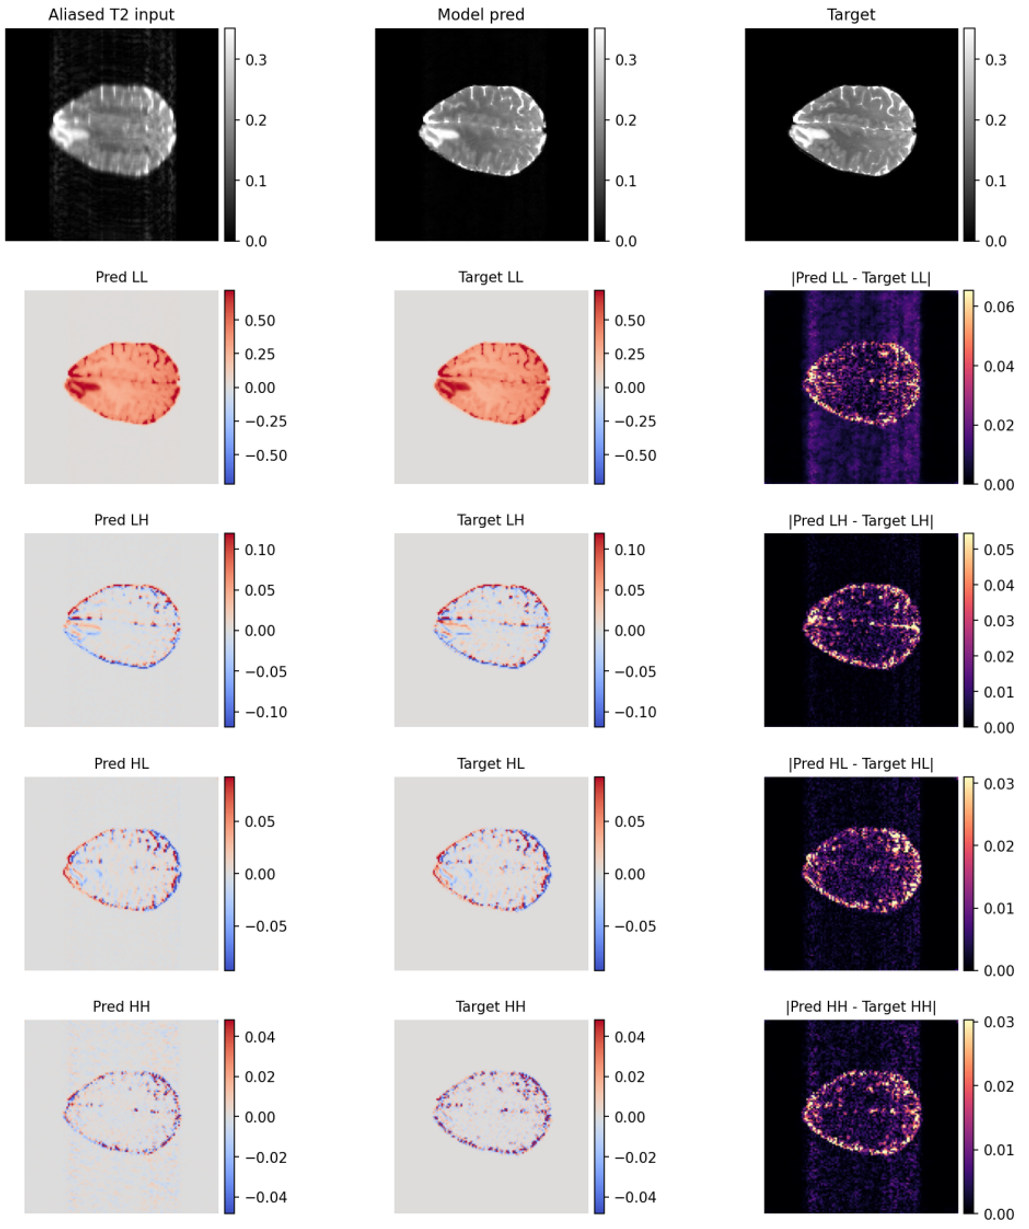
\includegraphics[width=0.8\linewidth]{figures/wavelet.png}
    \caption{Visualization of the Wavelet Loss components. The figure compares the predicted and target images across different frequency bands (LL, LH, HL, HH), highlighting the structural details captured by the high-frequency components.}
    \label{fig:wavelet_vis}
\end{figure}

\textbf{Perceptual Loss ($\mathcal{L}_{LPIPS}$):} To ensure the reconstructed image aligns with human visual perception and preserves complex texture details, we incorporated the Learned Perceptual Image Patch Similarity (LPIPS) metric as a loss function. This perceptual loss computes the distance between deep feature representations extracted by a pre-trained network, rather than simply comparing raw pixel intensities. 


\begin{figure*}[t] 
	\begin{center} 
		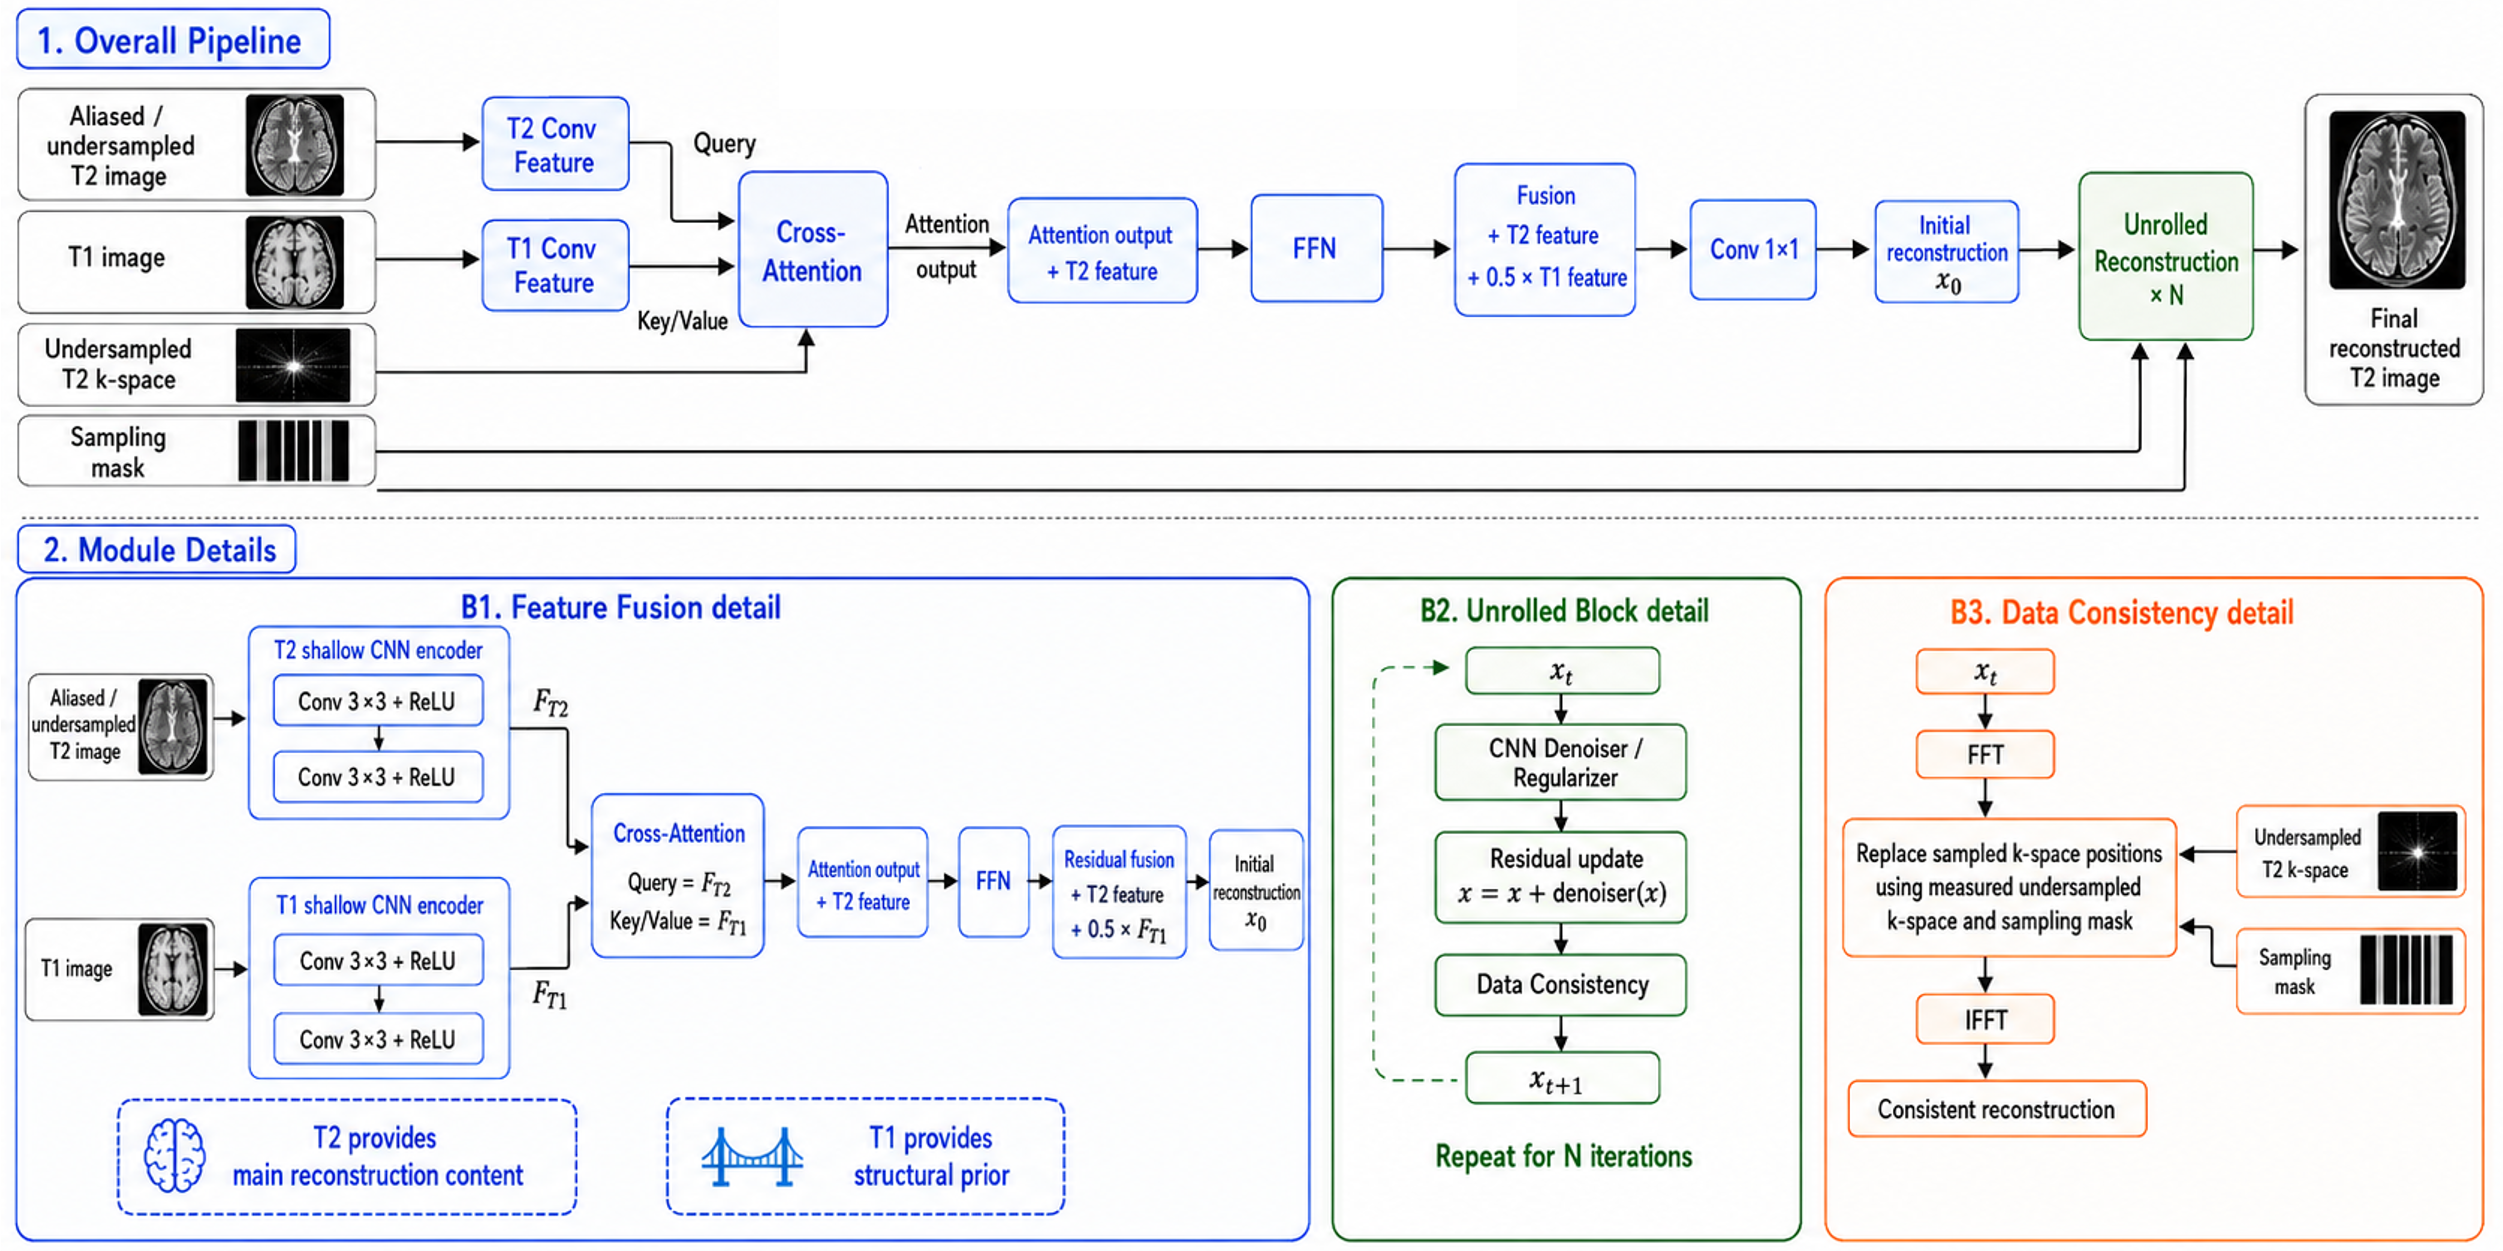
\includegraphics[width=\linewidth]{figures/pipeline_2.png} 
	\end{center} 
    \vspace{-20pt}  
	\caption{Overall pipeline of the Multi-modal Unrolled Reconstruction Network (Task 3).}
	\label{fig:task3_pipeline} 
	\vspace{-15pt}
\end{figure*}
\section{IMPLEMENTATION DETAILS}
\label{sec:implementation_details}

\subsection{Data Preprocessing}
\label{sec:data_preprocessing}

We preprocess the BraTS data at the patient level, where each subject contains multi-modal 3D NIfTI volumes. In our current local copy, the dataset contains 625 subjects. For each subject, we load the T2-weighted volume (\texttt{t2w}) as the reconstruction target modality and the native T1-weighted volume (\texttt{t1n}) as the auxiliary anatomical modality. Both volumes are converted to \texttt{float32} and transposed into a slice-first representation of shape $(D, H, W)$.

Each 3D volume is independently normalized to $[0,1]$ using min-max normalization. We further discard nearly empty boundary slices using a low-variance threshold.

To emulate accelerated MRI acquisition, we transform each fully sampled T2 slice to k-space and apply a variable-density Cartesian undersampling mask. Unless otherwise stated, we use an acceleration factor of $R=5$ with center fraction $0.08$. The inverse FFT magnitude is used as the aliased T2 input.

For each retained slice, we store the aliased T2 image, the fully sampled T2 image, the fully sampled T1 image, the undersampling mask, and the undersampled complex k-space.

We split the dataset at the patient level to avoid leakage across slices from the same subject. Specifically, subjects are randomly shuffled with seed $42$ and divided into training, validation, and test sets with ratios of $70\%$, $15\%$, and $15\%$, respectively. Under the current dataset size of 625 subjects, this produces 437 training subjects, 93 validation subjects, and 95 test subjects.

\subsection{U-Net (Task2) Training Settings}
\label{sec:unet_training_settings}

For Task 2, we train a baseline single-modal U-Net reconstructor on the preprocessed dataset. The network takes the aliased T2 slice as input and predicts the fully sampled T2 slice in the image domain.

The baseline model is a standard encoder-decoder U-Net with depth $4$ and base width $16$.

We optimize the model using MSE loss and Adam with learning rate $1\times10^{-3}$. Training runs for $50$ epochs with batch size $128$, and validation is performed every epoch.

We use a short warmup stage followed by \texttt{ReduceLROnPlateau} learning-rate decay, together with gradient clipping and early stopping.

During evaluation, we report NMSE, PSNR, SSIM, and LPIPS.

We keep the best checkpoint according to validation loss.

\subsection{Multi-modal Unrolled Reconstruction Network (Task3) Training Settings}
\label{sec:multimodal_unrolled_training_settings}

For Task 3, we train a multi-modal unrolled reconstruction network on the same preprocessed dataset. The model takes the aliased T2 image, fully sampled T1 image, undersampling mask, and undersampled T2 k-space as inputs, and predicts the fully sampled T2 image.

The model uses a T1-guided unrolled architecture with $5$ iterations. Each iteration consists of a learned denoising block followed by a hard data-consistency step in k-space. In our main setting, the denoiser width is $32$ channels.

The training objective combines MSE loss, Haar high-frequency wavelet loss, and LPIPS perceptual loss, with weights $1.0$, $0.03$, and $0.1$, respectively. We train the model with Adam for $80$ epochs using batch size $32$ and gradient accumulation over $2$ steps, giving an effective batch size of $64$. The initial learning rate is $1.5\times10^{-4}$.

We use one-epoch warmup followed by \texttt{ReduceLROnPlateau} learning-rate decay, together with gradient clipping and mixed-precision training.

Validation is performed every epoch, and we report NMSE, PSNR, SSIM, and LPIPS.

We keep the best checkpoint according to validation loss.

















% \begin{figure*}[htbp] 
% 	\begin{center} 
% 		\includegraphics[width=0.99\linewidth]{figures/comparison1.jpg} 
% 	\end{center} 
% 	\vspace{-16pt}
% 	\caption{Qualitative comparison with SOTA playback-only methods on novel view synthesis on DualGS dataset.}
% 	\label{fig:fig_comp_1}
% \end{figure*} 


% \begin{figure*}[htbp] 
% 	\begin{center} 
% 		\includegraphics[width=0.99\linewidth]{figures/comparison2.jpg} 
% 	\end{center} 
% 	\vspace{-16pt}
% 	\caption{Qualitative comparison with AP-NeRF~\cite{uzolas2024template}, TAVA~\cite{li2022tava} and SC-GS~\cite{huang2024sc} on both training motion and novel motion synthesis.}
%         \vspace{-16pt}
% 	\label{fig:fig_comp_2}
% \end{figure*} 


\section{Experimental Results} 

\subsection{Quantitative Comparison: Task 2 vs. Task 3}
\begin{figure*}[t]
    \centering
    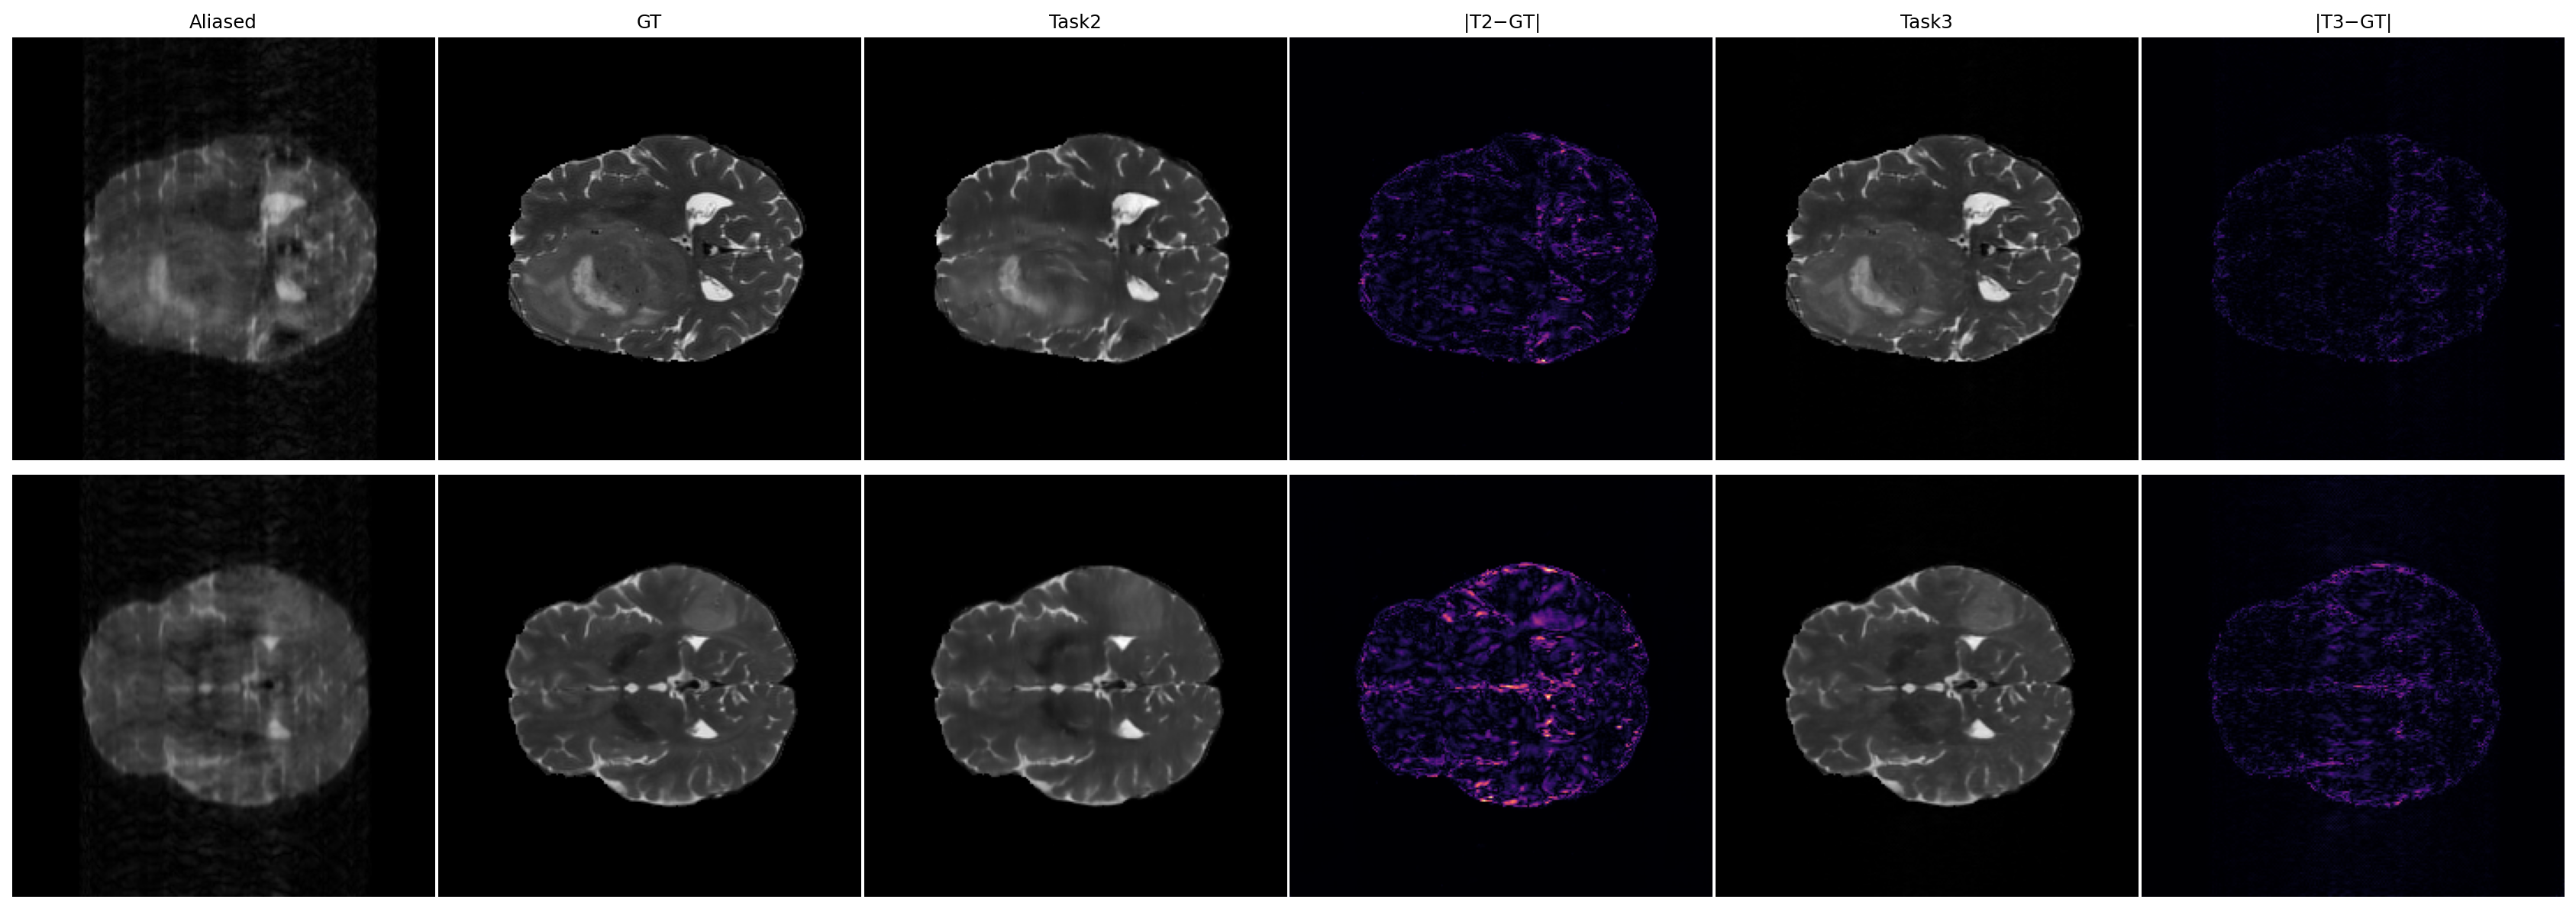
\includegraphics[width=\textwidth]{figures/task2_task3_two_case_paper_grid.png}
    \caption{Qualitative comparison of reconstruction results between Task 2 and Task 3.}
    \label{fig:qualitative_results}
\end{figure*}

To comprehensively evaluate the reconstruction performance of the baseline U-Net (Task 2) and the proposed Multi-modal Unrolled Network (Task 3), we adopted four complementary metrics, including Peak Signal-to-Noise Ratio (PSNR), Structural Similarity Index Measure (SSIM), Learned Perceptual Image Patch Similarity (LPIPS), and Deep Image Structure and Texture Similarity (DISTS). While PSNR and SSIM mainly measure pixel-level fidelity and structural consistency, LPIPS and DISTS further evaluate perceptual similarity and texture preservation from a human visual perspective.

As summarized in Table~\ref{tab:main_results}, the proposed Task 3 framework consistently achieves superior performance across all evaluation metrics. Specifically, Task 3 improves PSNR from 37.21 dB to 41.11 dB and increases SSIM from 0.885 to 0.954, demonstrating substantially better reconstruction accuracy and structural consistency. Meanwhile, LPIPS decreases from 0.0205 to 0.0090 and DISTS decreases from 0.1558 to 0.0936, indicating that the proposed method produces reconstructions with significantly improved perceptual quality and more realistic texture recovery.

The qualitative comparisons in Figure~\ref{fig:qualitative_results} further support these observations. Compared with the baseline Task 2 results, the Task 3 reconstructions exhibit sharper anatomical boundaries, clearer tumor structures, and fewer residual artifacts. Moreover, the corresponding error maps ($|T2-GT|$ and $|T3-GT|$) reveal that the proposed method significantly suppresses reconstruction errors, particularly around fine structural details and high-frequency regions. These improvements demonstrate the effectiveness of incorporating multi-modal priors together with iterative data consistency refinement in the unrolled reconstruction framework.

\begin{table}[h]
\centering
\caption{Quantitative comparison between Task 2 (Baseline) and Task 3 (Multi-modal Unrolled Network).}
\label{tab:main_results}
% 将表格宽度缩放为当前行宽 (列宽) 的 90%。高度设为 ! 表示保持原本的长宽比。
\resizebox{1.0\linewidth}{!}{
\begin{tabular}{lcccc}
\toprule
\textbf{Model} & \textbf{DISTS} $\downarrow$ & \textbf{LPIPS} $\downarrow$ & \textbf{PSNR} $\uparrow$ & \textbf{SSIM} $\uparrow$ \\
\midrule
Task 2 (U-Net) & 0.1558 & 0.0205 & 37.21 & 0.885 \\
Task 3 (Proposed) & 0.0936 & 0.0090 & 41.11 & 0.954 \\
\bottomrule
\end{tabular}
}
\end{table}

\subsection{Qualitative Results and Training Logs}

Figure~\ref{fig:random_sampled_worst_distinct_patients_paper_figure} shows the five worst Task 3 cases ranked by PSNR. Despite severe aliasing in the inputs, the reconstructions preserve the main anatomical structures and lesion regions, demonstrating the robustness of the proposed model on challenging samples. Remaining errors mainly appear as mild over-smoothing of fine textures and residual boundary artifacts, especially near cortical folds, tumor margins, and image borders.

Figure~\ref{fig:training_logs_1} shows the validation curves of the Task 2 baseline. The validation loss and NMSE decrease rapidly in the early training stage and then gradually converge, while PSNR and SSIM increase and stabilize. This indicates that the baseline U-Net learns a reasonable reconstruction mapping from undersampled inputs. However, the PSNR and SSIM curves exhibit noticeable early-stage fluctuations, suggesting that the baseline remains less stable on challenging validation samples.

Figure~\ref{fig:training_logs_2} further reports the Task 3 training dynamics. The training and validation losses decrease rapidly in the early epochs and then gradually stabilize, suggesting effective optimization without obvious overfitting. Meanwhile, PSNR increases steadily, while LPIPS and DISTS decrease, indicating simultaneous improvements in pixel fidelity, perceptual similarity, and structural texture preservation.

Overall, the qualitative results and training logs are consistent with Table~\ref{tab:main_results}. Task 3 produces sharper and more faithful reconstructions than the Task 2 baseline, while the remaining failures are mainly concentrated in fine anatomical details, lesion boundaries, and image-edge artifacts.

\begin{figure}[h]
    \centering
    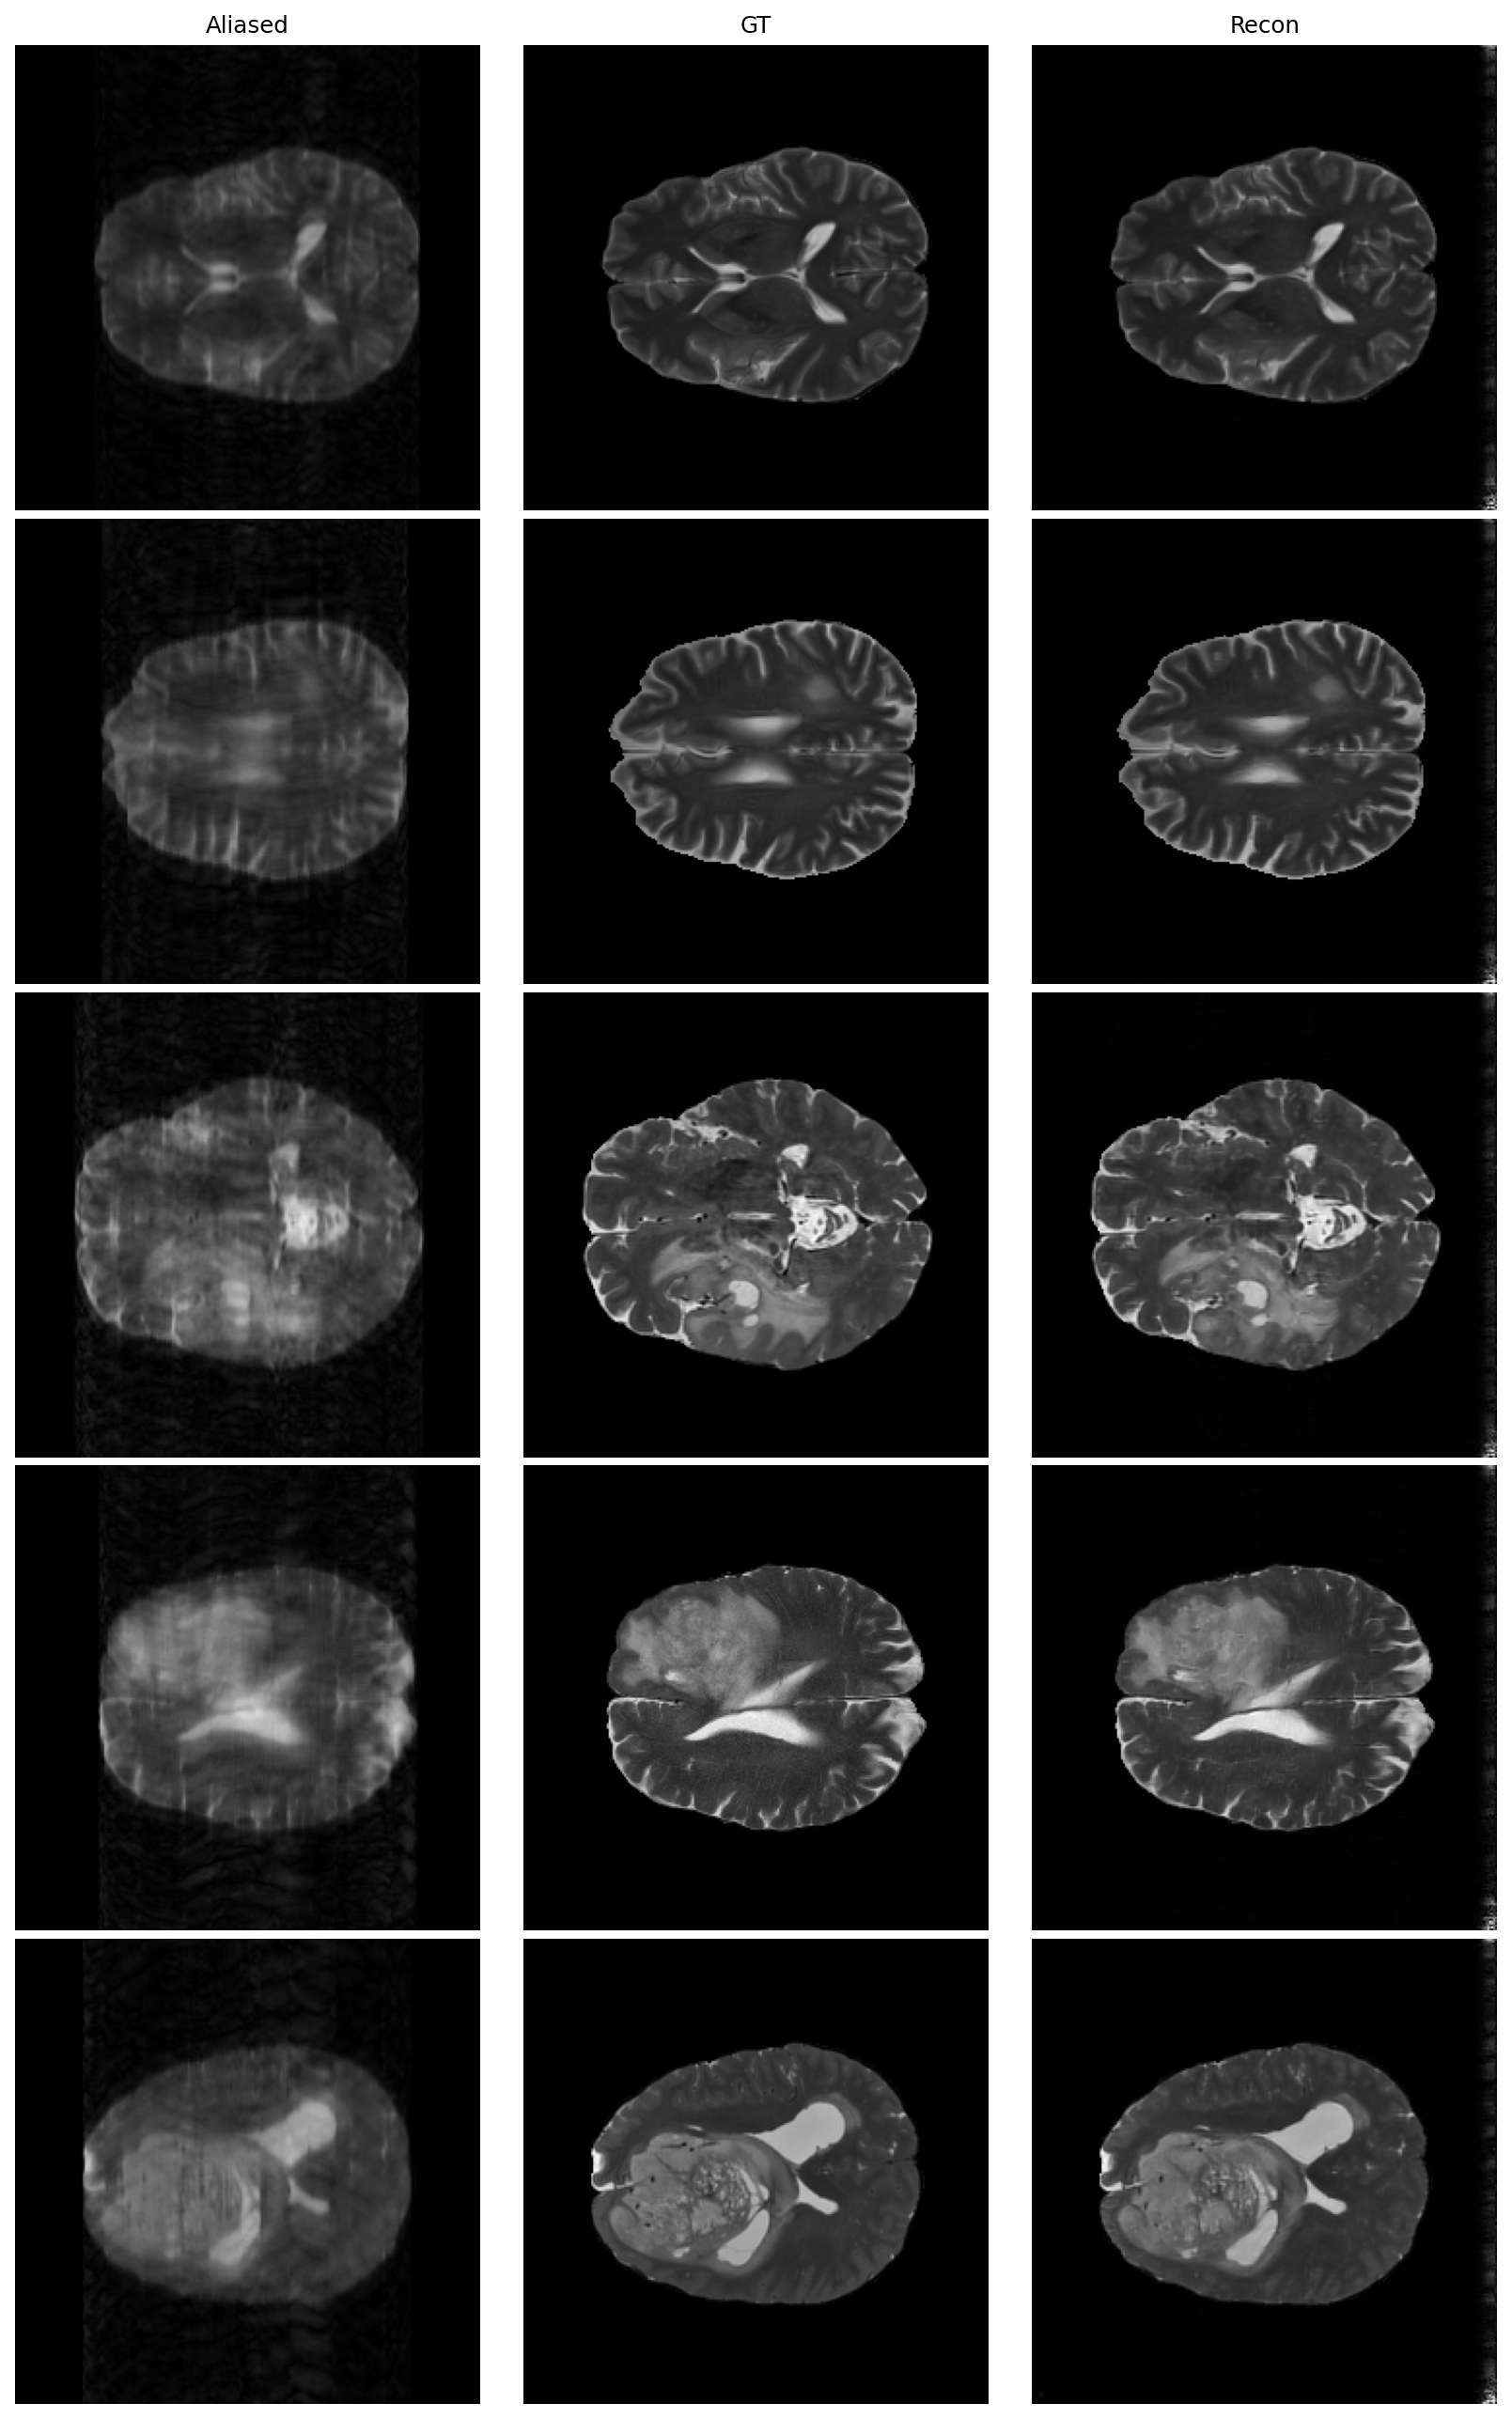
\includegraphics[width=\linewidth]{figures/random_sampled_worst_distinct_patients_paper_figure.png}
    \caption{The five worst-performing reconstruction cases from the task3 baseline (calculated using PSNR as the metric).}
    \label{fig:random_sampled_worst_distinct_patients_paper_figure}
\end{figure}

\begin{figure}[h]
    \centering
    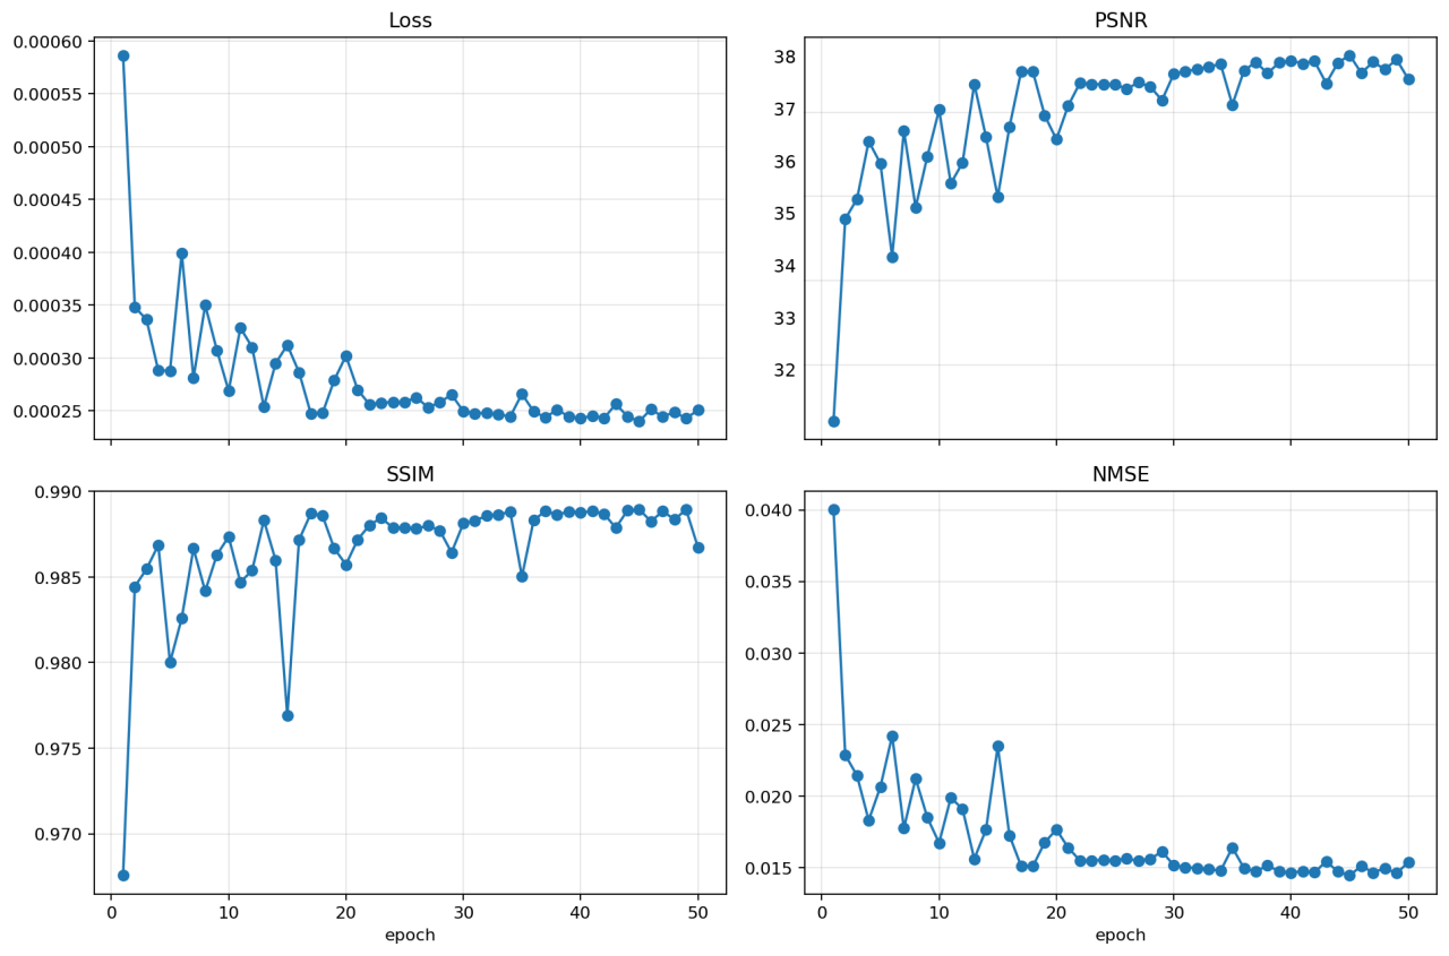
\includegraphics[width=\linewidth]{figures/training_logs_1.png}
    \caption{Validation loss curves for Task 2.}
    \label{fig:training_logs_1}
\end{figure}

\begin{figure}[h]
    \centering
    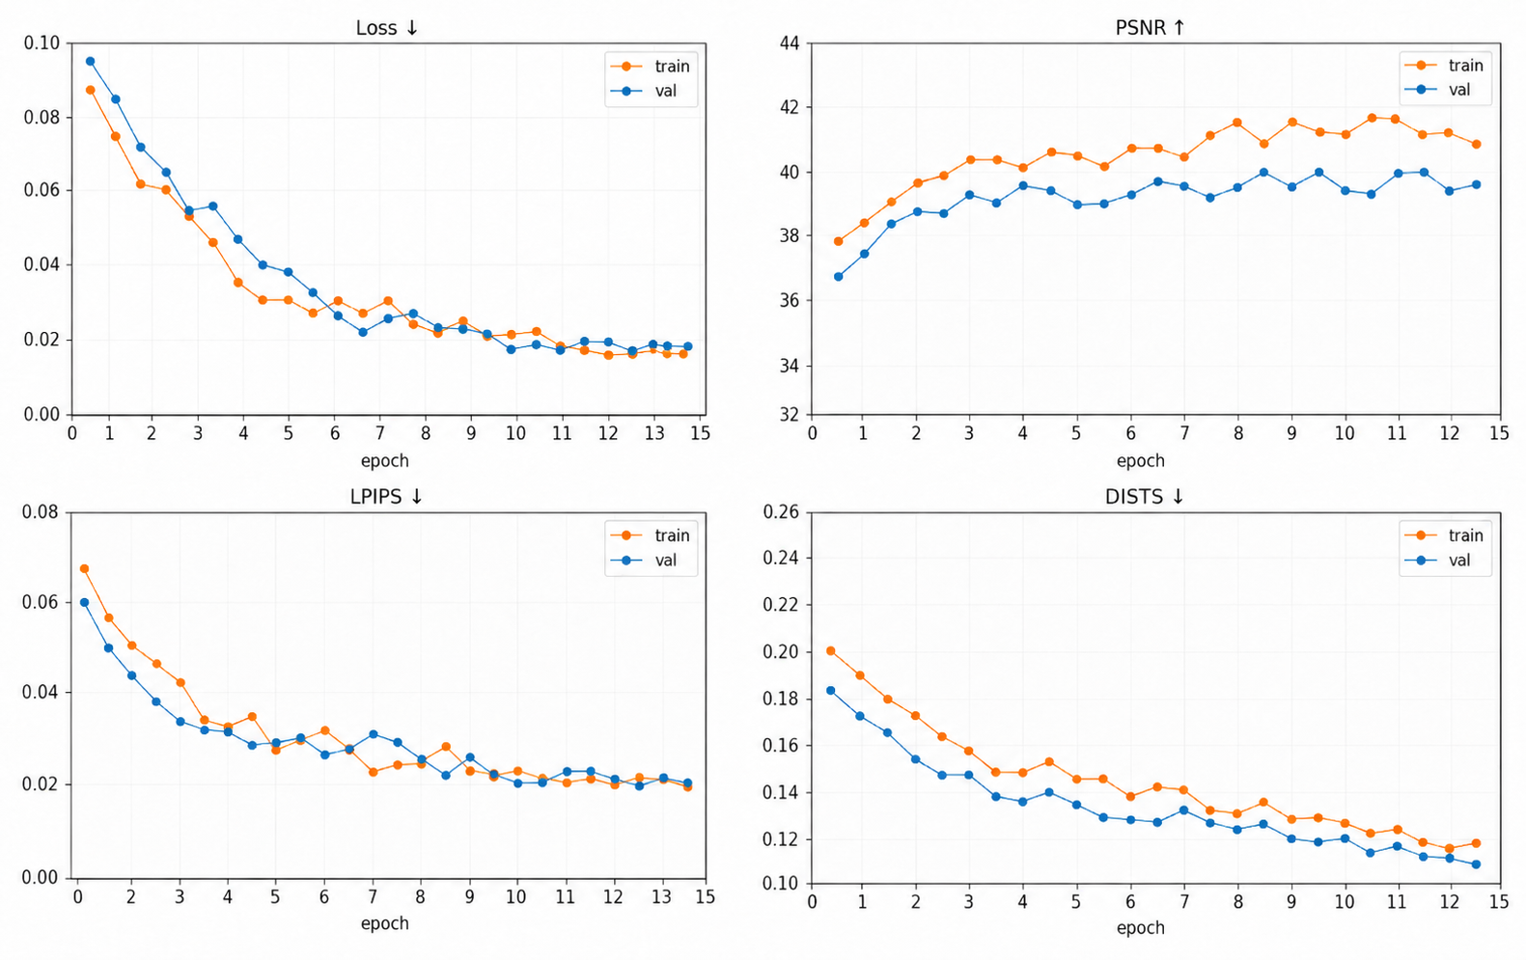
\includegraphics[width=\linewidth]{figures/training_logs_2.png}
    \caption{Training and Validation loss curves for Task 3.}
    \label{fig:training_logs_2}
\end{figure}

\subsection{Rethinking PSNR: Alignment with Human Perception}
During our initial analysis of the Task 2 results, we encountered a significant contradiction: images with higher PSNR values did not consistently yield better subjective visual quality. As illustrated in Figure \ref{fig:psnr_error}, Slice 43 achieves a higher PSNR (39.10 dB) than Slice 28 (35.34 dB). However, inspecting the Error Maps and the perceptual LPIPS metric reveals the opposite story: Slice 43 has a significantly worse LPIPS score (0.0364 vs. 0.0194) and exhibits denser, more structured errors, aligning better with human visual dissatisfaction.

\begin{figure}[h]
    \centering
    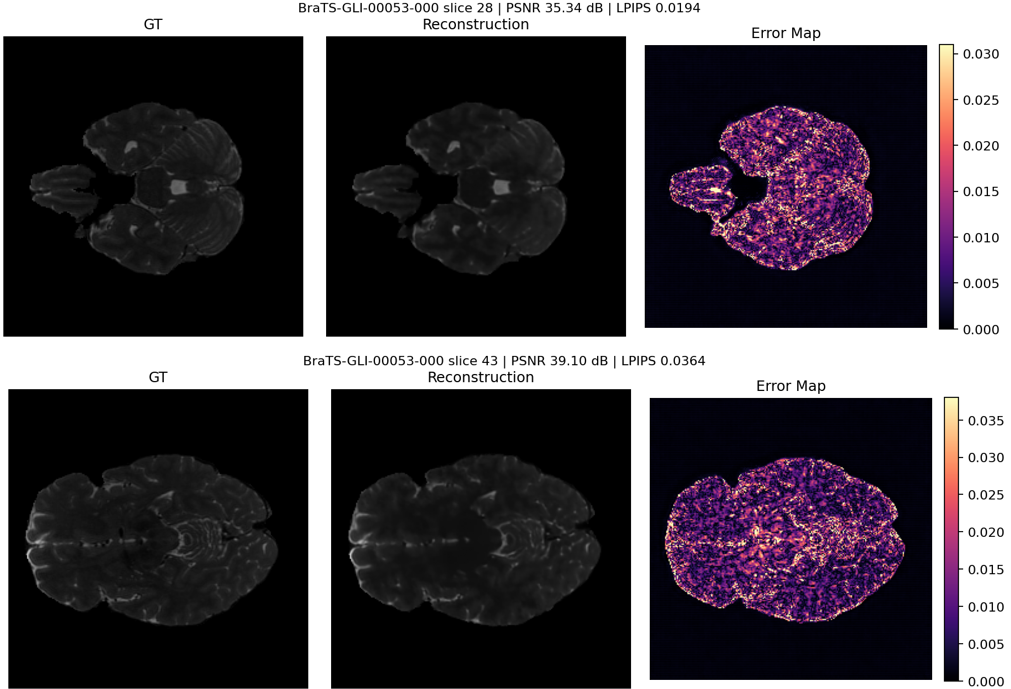
\includegraphics[width=\linewidth]{figures/PNSR.png}
    \caption{Contradiction between PSNR and Perceptual Quality. Slice 43 (bottom) has a higher PSNR but a noticeably worse Error Map and LPIPS score compared to Slice 28 (top).}
    \label{fig:psnr_error}
\end{figure}

To systematically investigate this metric failure, we drew inspiration from the supplemental materials of Apple's research on image sharpness \cite{mescheder2025sharp}. We conducted a ``shifting pixels'' experiment by translating the reference MRI image by minor spatial percentages. 

\begin{figure}[h]
    \centering
    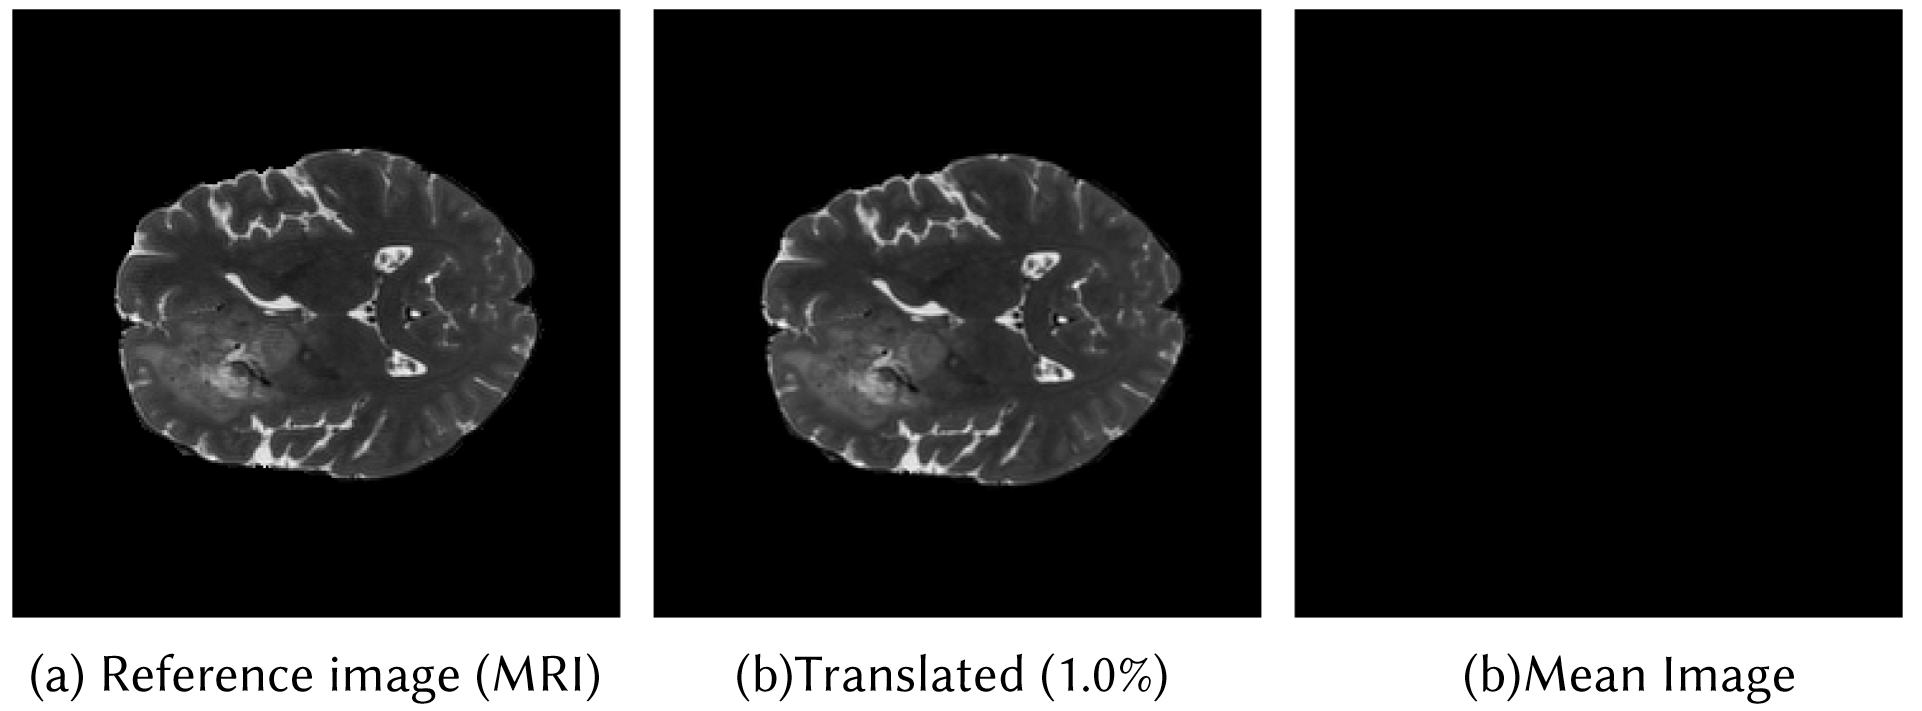
\includegraphics[width=\linewidth]{figures/PSNR_exp.png}
    \caption{The translation experiment. A visually identical translated image suffers massive PSNR degradation compared to the reference.}
    \label{fig:translation_vis}
\end{figure}

As shown in Figure \ref{fig:translation_vis} and detailed in Table \ref{tab:translation_exp}, shifting the image by merely 1.0\% causes the PSNR to plummet drastically to 20.9 dB, a score typically associated with severe degradation. Yet, to the human eye, the 1.0\% translated image is nearly indistinguishable from the reference. In contrast, perceptual metrics like DISTS and LPIPS remain relatively stable and robust to these imperceptible shifts. This experiment definitively proves that purely pixel-aligned metrics like PSNR and MSE heavily penalize slight spatial misalignments while ignoring structural integrity, justifying our critical decision to incorporate Wavelet and Perceptual (LPIPS/DISTS) losses into our final Task 3 pipeline.

\begin{table}[h]
\centering
\caption{Results of the spatial translation experiment on evaluation metrics. Perceptual metrics (DISTS, LPIPS) degrade gracefully, whereas pixel-wise metrics (PSNR, SSIM) collapse under minor shifts.}
\label{tab:translation_exp}
% 使用 resizebox 缩放表格，0.9\linewidth 表示缩放到行宽的 90%
\resizebox{1.0\linewidth}{!}{
\begin{tabular}{lcccc}
\toprule
\textbf{Comparison} & \textbf{DISTS} $\downarrow$ & \textbf{LPIPS} $\downarrow$ & \textbf{PSNR} $\uparrow$ & \textbf{SSIM} $\uparrow$ \\
\midrule
Translated (0.1\%) & 0.028 & 0.007 & 35.9 & 0.988 \\
Translated (1.0\%) & 0.073 & 0.059 & 20.9 & 0.760 \\
Translated (5.0\%) & 0.070 & 0.220 & 17.4 & 0.651 \\
Translated (15.0\%) & 0.120 & 0.422 & 15.2 & 0.538 \\
Mean Image         & 0.655 & 0.612 & 16.8 & 0.085 \\
\bottomrule
\end{tabular}
}
\end{table}

\subsection{Ablation Study}
To validate the individual contributions of our proposed hybrid loss components, we conducted a rigorous ablation study on our network. We incrementally added the Wavelet Loss and the Perceptual (LPIPS) Loss to the baseline MSE objective.


\begin{figure}[h]
    \centering
    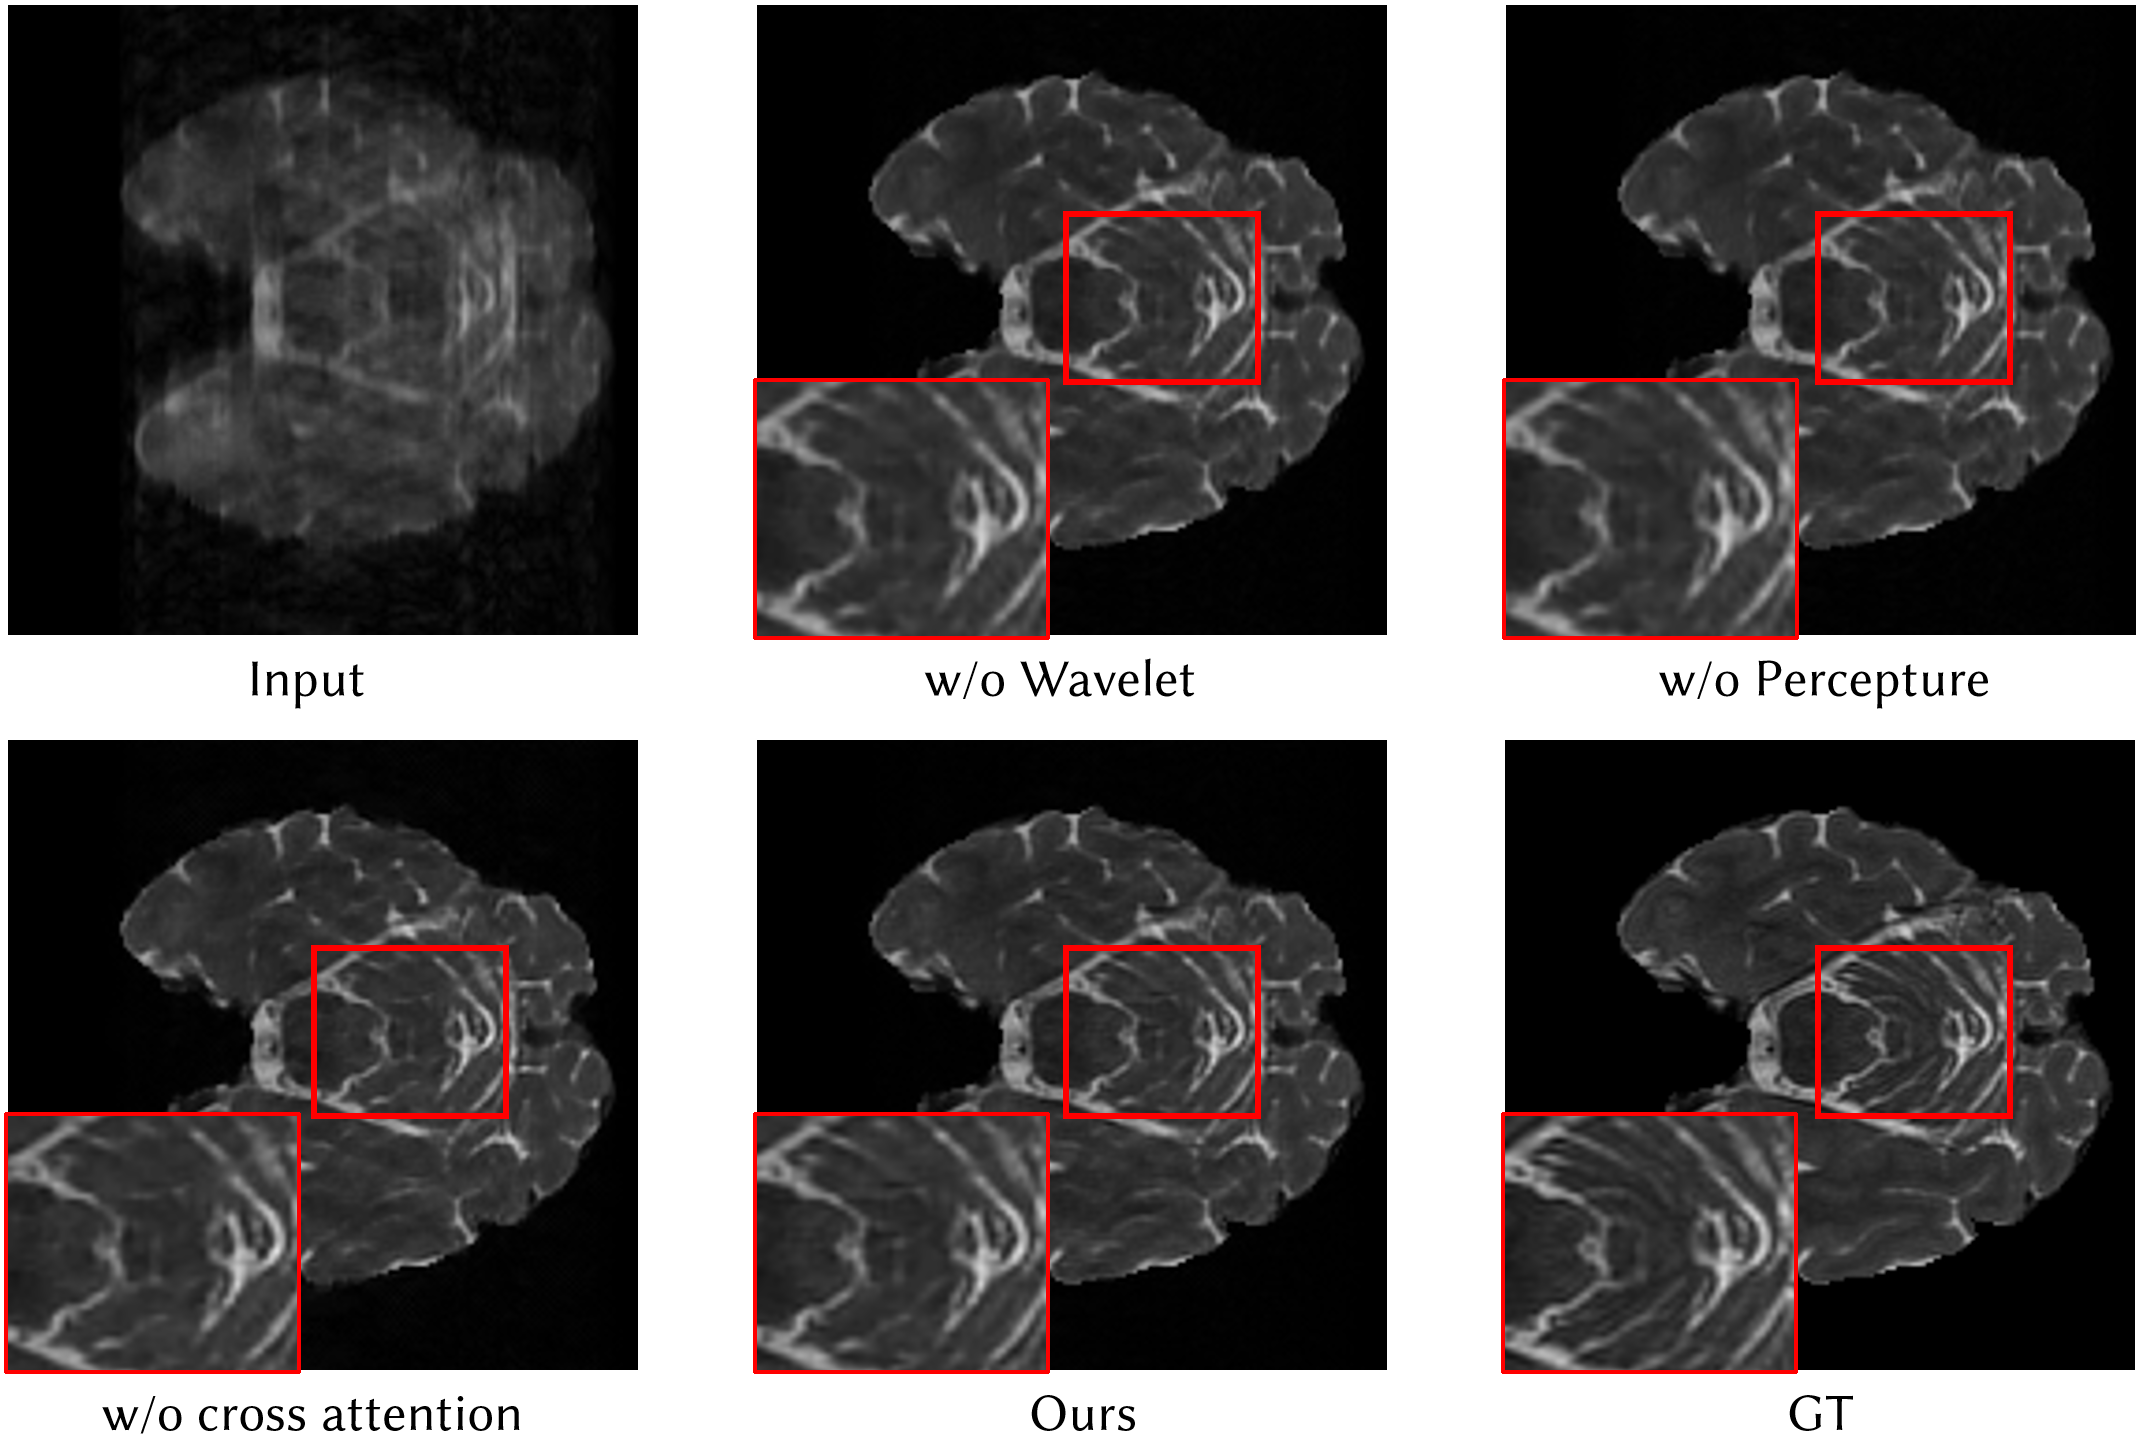
\includegraphics[width=\linewidth]{figures/ablation.png}
    \caption{Qualitative ablation study on key training components.}
    \label{fig:ablation_vis}
\end{figure}

\begin{table}[h]
\centering
\caption{Quantitative ablation results comparing the full proposed multi-modal model against simplified configurations.}
\label{tab:ablation_results}
\resizebox{1.0\linewidth}{!}{
\begin{tabular}{lcccc}
\toprule
\textbf{Configuration} & \textbf{DISTS} $\downarrow$ & \textbf{LPIPS} $\downarrow$ & \textbf{PSNR} $\uparrow$ & \textbf{SSIM} $\uparrow$ \\
\midrule
w/o Wavelet & 0.1289 & 0.0185 & 38.77 & 0.888 \\
w/o Perceptual & 0.1395 & 0.0198 & 37.56 & 0.885 \\
w/o Cross-Attention & 0.1334 & 0.0191 & 37.79 & 0.887 \\
\textbf{Ours (Task 3)} & \textbf{0.0936} & \textbf{0.0090} & \textbf{41.11} & \textbf{0.954} \\
\bottomrule
\end{tabular}
}
\end{table}

As observed in Table \ref{tab:ablation_results} and Figure \ref{fig:ablation_vis}, relying solely on MSE leads to over-smoothed textures. The addition of the Wavelet loss successfully recovers high-frequency edges, while the further integration of the Perceptual loss maximally restores the organic texture of the brain tissues, yielding the best overall DISTS and LPIPS scores.

% \begin{table}[t]
% 	\begin{center}
% 		\centering
% 		\vspace{20pt}

% 		\resizebox{0.47\textwidth}{!}{
% 			\begin{tabular}{l|cccc}
% 				\hline
% 				Method   &  PSNR $\uparrow$ & SSIM $\uparrow$ & LPIPS $\downarrow$ & Training Time(Min / frame) $\downarrow$ \\
% 				\hline
% 				NeuS2~\cite{wang2023neus2}\qquad\qquad & 29.589 & 0.967 & 0.0561 & 3.23  \\
% 			    Spacetime Gaussian~\cite{li2023spacetime}     & 31.691 & 0.981 & 0.0289 & 2.24  \\
%                 DualGS~\cite{jiang2024robust} & \bestCellColor{35.506} & \bestCellColor{0.990} & \secondBestCellColor{0.0193} & 12.22  \\
%                 $V^3$~\cite{wang2024v} & 33.821 & 0.984 & \bestCellColor{0.0167} & \secondBestCellColor{\textbf{1.86}}  \\
%     		\hline
%                 Ours & \secondBestCellColor{\textbf{34.571}} & \secondBestCellColor{\textbf{0.986}} & \textbf{0.0229} & \bestCellColor{\textbf{1.68}} \\
% 				\hline
% 			\end{tabular}
%             }
%             \caption{
%             Quantitative comparison of novel view rendering. Green and yellow cell colors indicate the best and the second-best results. %
%             }
% 		\label{table:Qualitativecomparison}
%         \vspace{-20pt}
% 	\end{center}
% \end{table}

% \begin{table}[t]
%     \centering

%     \resizebox{\columnwidth}{!}{ %
%     \begin{tabular}{c|c c c|c c c}
%         \hline
%         \multirow{2}{*}{\textbf{Methods}} & \multicolumn{3}{c|}{\textbf{Novel View}} & \multicolumn{3}{c}{\textbf{Novel Motion}} \\
%         & PSNR $\uparrow$ & SSIM $\uparrow$  &  LPIPS $\downarrow$ & PSNR $\uparrow$ & SSIM $\uparrow$  &  LPIPS $\downarrow$ \\
%         \hline
%         AP-NeRF ~\cite{uzolas2024template} & 28.26 & 0.939 & 0.0768 & \secondBestCellColor{26.85} & \secondBestCellColor{0.944} & \secondBestCellColor{0.0519} \\
%         TAVA~\cite{li2022tava}  & 21.57 & 0.906 &  0.1292& 21.34 & 0.905 & 0.1301 \\
%         SC-GS~\cite{huang2024sc}  & \secondBestCellColor{30.63} & \secondBestCellColor{0.971} & \secondBestCellColor{0.0319} & 19.18 & 0.907 & 0.0821 \\
%         \hline

%         Ours  & \bestCellColor{\textbf{32.09}} & \bestCellColor{\textbf{0.979}} & \bestCellColor{\textbf{0.0310}} & \bestCellColor{\textbf{30.06}} & \bestCellColor{\textbf{0.976}} & \bestCellColor{\textbf{0.0277}} \\
%         \hline
%     \end{tabular}
%     }
%     \caption{
%     Quantitative comparison with template-free modeling approaches in both novel views and motions. 
%     }
%     \label{table:Qualitativecomparison2}
% \end{table}

\section{Conclusion}

In this work, we studied multi-contrast MRI reconstruction from undersampled k-space data. We first established a single-modal U-Net baseline for Task 2, which effectively suppresses aliasing artifacts but tends to produce over-smoothed reconstructions. To overcome this limitation, we proposed a Multi-modal Unrolled Reconstruction Network for Task 3, which leverages the fully sampled T1 modality as anatomical guidance for undersampled T2 reconstruction. By combining cross-attention-based feature fusion, iterative unrolled refinement, and explicit k-space data consistency, the proposed method achieves more faithful and perceptually realistic reconstructions.

Extensive experiments show that our Task 3 model consistently outperforms the Task 2 baseline across PSNR, SSIM, LPIPS, and DISTS. Qualitative results further demonstrate that the proposed framework better preserves anatomical boundaries, tumor regions, and fine structural details while reducing residual undersampling artifacts. In addition, our analysis of PSNR reveals its limitation in reflecting perceptual image quality, motivating the use of perceptual and structure-aware metrics. The ablation study confirms the effectiveness of the proposed components, including wavelet loss, perceptual loss, and cross-attention-based multi-modal fusion.

Despite these improvements, challenging pathological cases still exhibit mild over-smoothing and boundary artifacts. Future work may explore stronger edge-aware constraints, more robust multi-modal registration, and advanced frequency-domain modeling. Overall, our results demonstrate that integrating multi-modal anatomical priors with unrolled data consistency and perceptually motivated objectives is an effective direction for high-quality accelerated MRI reconstruction.
\begin{thebibliography}{99}

\bibitem{lustig2007sparse}
Lustig, M., Donoho, D., and Pauly, J. M.
\newblock Sparse MRI: The application of compressed sensing for rapid MR imaging.
\newblock \emph{Magnetic Resonance in Medicine}, 58(6):1182--1195, 2007.

\bibitem{schlemper2018deep}
Schlemper, J., Caballero, J., Hajnal, J. V., Price, A. N., and Rueckert, D.
\newblock A deep cascade of convolutional neural networks for dynamic MR image reconstruction.
\newblock \emph{IEEE Transactions on Medical Imaging}, 37(2):491--503, 2018.

\bibitem{wang2016accelerating}
Wang, S., Su, Z., Ying, L., Peng, X., Zhu, S., Liang, F., Feng, D., Liang, D.
\newblock Accelerating magnetic resonance imaging via deep learning.
\newblock In \emph{2016 IEEE 13th International Symposium on Biomedical Imaging (ISBI)}, pages 514--517, 2016.

\bibitem{ronneberger2015u}
Ronneberger, O., Fischer, P., and Brox, T.
\newblock U-Net: Convolutional networks for biomedical image segmentation.
\newblock In \emph{Medical Image Computing and Computer-Assisted Intervention -- MICCAI 2015}, pages 234--241, 2015.

\bibitem{johnson2016perceptual}
Johnson, J., Alahi, A., and Fei-Fei, L.
\newblock Perceptual losses for real-time style transfer and super-resolution.
\newblock In \emph{European Conference on Computer Vision (ECCV)}, pages 694--711, 2016.

\bibitem{ledig2017photo}
Ledig, C., Theis, L., Husz{\'a}r, F., Caballero, J., Cunningham, A., Acosta, A., Aitken, A., Tejani, A., Totz, J., Wang, Z., and Shi, W.
\newblock Photo-realistic single image super-resolution using a generative adversarial network.
\newblock In \emph{Proceedings of the IEEE Conference on Computer Vision and Pattern Recognition (CVPR)}, pages 4681--4690, 2017.

\bibitem{kang2018deep}
Kang, E., Min, J., and Ye, J. C.
\newblock Wavelet domain residual network (WavResNet) for low-dose X-ray CT reconstruction.
\newblock \emph{IEEE Transactions on Medical Imaging}, 37(12):2986--2997, 2018.

\bibitem{ding2022image}
Ding, K., Ma, K., Wang, S., and Simoncelli, E. P.
\newblock Image quality assessment: Unifying structure and texture similarity.
\newblock \emph{IEEE Transactions on Pattern Analysis and Machine Intelligence}, 44(5):2567--2581, 2022.

\bibitem{zhou2020dudornet}
Zhou, B. and Zhou, S. K.
\newblock DuDoRNet: Learning a dual-domain recurrent network for fast MRI reconstruction with deep T1 prior.
\newblock In \emph{Proceedings of the IEEE/CVF Conference on Computer Vision and Pattern Recognition (CVPR)}, pages 4273--4282, 2020.

\bibitem{mescheder2025sharp}
Mescheder, L., Dong, W., Li, S., Bai, X., Santos, M., Hu, P., Lecouat, B., Zhen, M., Delaunoy, A., Fang, T., Tsin, Y., Richter, S. R., and Koltun, V.
\newblock Sharp monocular view synthesis in less than a second.
\newblock \emph{arXiv preprint arXiv:2512.10685}, 2025.

\end{thebibliography}

% \bibliographystyle{ieeenat_fullname}
% \bibliography{reference}


\end{document}
